\documentclass{article}
\usepackage{amsmath,amsthm,amsfonts,amssymb,fullpage,graphicx}

\newtheorem{problem}{Problem}

\begin{document}

\begin{flushright}
Kris Harper\\

STAT 24400\\

October 7, 2010
\end{flushright}

\begin{center}
Homework 1
\end{center}

\begin{problem}
Verify the following extension of the addition rule (a) by an appropriate Venn diagram and (b) by a formal argument using the axioms of probability and the propositions in this chapter.
\[
P(A \cup B \cup C) = P(A) + P(B) + P(C) - P(A \cap B) - P(A \cap C) + P(B \cap C) + P(A \cap B \cap C).
\]
\end{problem}
\begin{proof}
(a) In the following Venn diagram we see that taking $A \cup B \cup C$ double counts the elements in $A \cap B$, $A \cap C$ and $B \cap C$ so we must subtract these from the total. But then we've clearly subtracted $A \cap B \cap C$ once too much, so we must add it back. This gives the formula.
\begin{center}
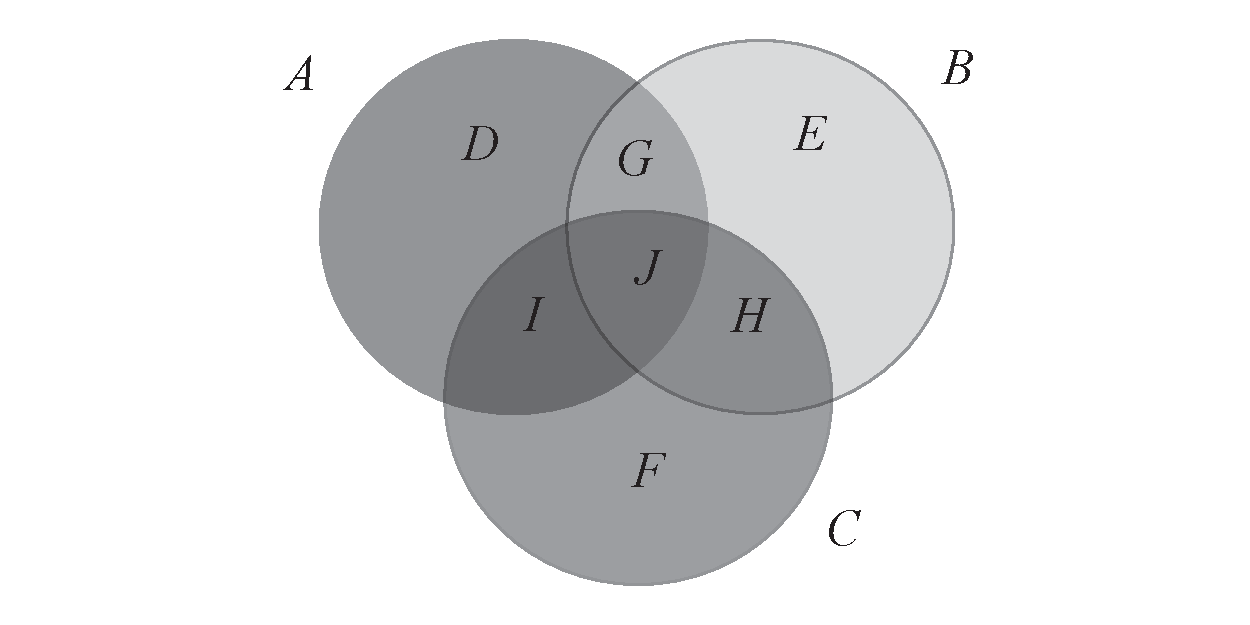
\includegraphics[width=300pt]{diagram.pdf}
\end{center}
(b) Let $D = A \cap (B \cup C)^c$, $E = B \cap (A \cup C)^c$, $F = C \cap (A \cap B)^c$, $G = A \cap B \cap C^c$, $H = B \cap C \cap A^c$, $I = A \cap C \cap B^c$ and $J = A \cap B \cap C$. Note that these sets are disjoint from each other. Note also that $A = D \cup G \cup I \cup J$, $B = E \cup G \cup H \cup J$ and $C = F \cup I \cup H \cup J$. Then
\begin{align*}
P(A \cup B \cup C)
&= P(D \cup E \cup F \cup G \cup H \cup I \cup J)\\
&= P(D \cup G \cup I \cup J) + P(E) + P(H) + P(F)\\
&= P(A) + P(E) + P(H) + P(F) + (P(G) + P(J) - P(G) - P(J))\\
&= P(A) + P(E \cup H \cup J \cup G) + P(F) - P(G) - P(J)\\
&= P(A) + P(B) + P(F) - P(J) - P(G) + (P(H) + P(I) + P(J) - P(H) - P(I) - P(J))\\
&= P(A) + P(B) + P(F \cup H \cup I \cup J) - P(J) - P(G) - P(H) - P(I) - P(J)\\
&= P(A) + P(B) + P(C) - P(G \cup J) - P(H \cup J) - P(I)\\
&= P(A) + P(B) + P(C) - P(A \cap B) - P(B \cap C) - P(I) + (P(J) - P(J))\\
&= P(A) + P(B) + P(C) - P(A \cap B) - P(B \cap C) - P(I \cup J) + P(J)\\
&= P(A) + P(B) + P(C) - P(A \cap B) - P(B \cap C) - P(A \cap C) + P(A \cap B \cap C)\\
\end{align*}
\end{proof}

\begin{problem}
Prove that
\[
P \left ( \bigcup_{i=1}^{n} A_i \right ) \leq \sum_{i=1}^{n} P(A_i).
\]
\end{problem}
\begin{proof}
We induct on $n$. The statement is clearly true for $n=1$. Suppose it's true for some positive integer $n$. Now, by the addition rule,
\begin{align*}
P \left (\bigcup_{i=1}^{n+1} A_i \right )
&= P \left ( \bigcup_{i=1}^{n} A_i \right ) + P(A_{n+1}) - P \left ( \left ( \bigcup_{i=1}^{n} A_i \right ) \cap A_{n+1} \right )\\
&\leq P \left ( \bigcup_{i=1}^{n} A_i \right ) + P(A_{n+1})\\
&\leq \sum_{i=1}^{n} P(A_i) + P(A_{n+1})\\
&= \sum_{i=1}^{n+1} P(A_i).
\end{align*}
Thus if the statement is true for $n$, it's also true for $n+1$ and we're done.
\end{proof}

\begin{problem}
The first three digits of a university telephone exchange are $452$. If all the sequences of the remaining four digits are equally likely, what is probability that a randomly selected university phone number contains seven distinct digits?
\end{problem}

There are $10$ possible values for each of the four remaining digits, so there are $10^4 = 10,000$ possible phone numbers. If we're to have $7$ distinct digits, none of the remaining digits can be $4$, $5$ or $2$ and they each must be distinct from each other. Thus there are $7$ possible values for the fourth digit, $6$ for the fifth, $5$ for the sixth and $4$ for the seventh. This gives a total of $7*6*5*4 = 840$ possible distinct numbers. Therefore the probability of getting such a number is $840/10,000 = .084$.

\begin{problem}
The four players in a bridge game are each dealt $13$ cards. How many ways are there to do this?
\end{problem}

We are grouping $52$ objects into $4$ classes with $13$ objects in each class. Therefore the ways to do this is
\[
\binom{52}{13 \; 13 \; 13 \; 13} = \frac{52!}{13!*13!*13!*13!} \approx 5.36 \times 10^{28}.
\]

\begin{problem}
How many difference letter arrangements can be obtained from the letters of the word \emph{statistically}, using all the letters?
\end{problem}

The word has $13$ letters so there are $13!$ arrangements. But there are two `s's, three `t's, two `a's, two `i's and two `l's. To compensate, we divide out by the permutations these letters could generate. This gives
\[
\frac{13!}{2!*3!*2!*2!*2!} = 64,864,800.
\]

\begin{problem}
A lot of $n$ items contains $k$ defectives, and $m$ are selected randomly and inspected. How should the value of $m$ be chosen so that the probability that at least one defective item turns up is $.90$? Apply your answer to (a) $n = 1,000$, $k = 10$, and (b) $n = 10,000$, $k = 100$.
\end{problem}

Let $A$ be the event that no defectives turn up. Then
\[
P(A) = \frac{\binom{n-k}{m} \binom{k}{0}}{\binom{n}{m}} = \frac{(n-k)!}{(n-k-m)!m!} \frac{k!}{k!} \frac{(n-m)!m!}{n!}
\]
which is the number of ways of choosing $m$ items from the $n-k$ good ones and $0$ items from the $k$ bad ones divided by the number of ways to choose $m$ items total. Simplifying the term on the right, we have
\[
\frac{(n-k)(n-k-1) \dots (n-k-m+1)}{(n)(n-1) \dots (n-m+1)}.
\]
If we assume $n$ is large in relation $k$ then this expression approximates as
\[
\left ( \frac{n-k}{n} \right )^m.
\]
We wish to find a value of $m$ such that
\[
P(A) \approx \left ( \frac{n-k}{n} \right )^m \leq .1.
\]
Taking $\log$ of both sides gives
\[
m \approx \frac{\log(.1)}{\log(n-k) - \log(n)}.
\]
(a) Putting in $n = 1,000$ and $k = 10$ gives
\[
m \approx \frac{\log(.1)}{\log(1000-10) - \log(1000)} \approx 229.1.
\]
(b) Putting in $n = 10,000$ and $k = 100$ gives
\[
m \approx \frac{\log(.1)}{\log(10000-100) - \log(10000)} \approx 229.1.
\]

\begin{problem}
A group of $60$ second graders is to be randomly assigned to two classes of $30$ each. (The random assignment is ordered by the school district to ensure against any bias.) Five of the second graders, Marcelle, Sarah, Michelle, Katy and Camerin, are close friends. What is the probability that they will all be in the same class? What is the probability that exactly four of them will be? What is the probability that Marcelle will be in one class and her friends in the other?
\end{problem}

The number of ways to pick $5$ students out of $60$ is $\binom{60}{5}$. The fact that there are two possible classes for the five friends to be in doubles the probability. Thus the probability of all five being in the same class is
\[
2 \frac{1}{\binom{60}{5}} \approx 3.66 \times 10^{-7}.
\]
If there are to be exactly four of the friends then there are $\binom{5}{4} = 5$ ways to pick four of the five friends, and $55$ possible students to fill the fifth slot. Thus there are
\[
2 * 5 * 55 \frac{1}{\binom{60}{5}} \approx 1.00 \times 10^{-4}.
\]
This is the same as the previous part, except that now we can't choose any four friends, so it's simply a fifth of the previous probability, or
\[
2 * 55 \frac{1}{\binom{60}{5}} \approx 2.01 \times 10^{-5}.
\]

\begin{problem}
Prove the following identity:
\[
\sum_{k=0}^{n} \binom{n}{k} \binom{m-n}{n-k} = \binom{m}{n}.
\]
\end{problem}
\begin{proof}
Suppose we have a collection of $m$ items. The number of ways to choose $n$ items from this set is $\binom{m}{n}$. Now let $0 \leq k \leq n$. Suppose we choose $k$ items from $n$ items in our collection. There are $\binom{n}{k}$ ways to do this. In order to pick a total of $n$ items, we must now pick $n-k$ items from the remaining $m-n$ items. There are $\binom{m-n}{n-k}$ ways to do this. If we multiply these two numbers we will get all possible combinations for picking $n$ items from $m$ items with that value of $k$. Now we let $k$ range over all possible values and then take a sum. This gives us
\[
\sum_{k=0}^{n} \binom{n}{k} \binom{m-n}{n-k} = \binom{m}{n}.
\]
\end{proof}

\begin{problem}
Urn $A$ has three red balls and two white balls, and urn $B$ has two red balls and five white balls. A fair coin is tossed. If it lands heads up, a ball is drawn from urn $A$; otherwise, a ball is drawn from urn $B$.\\
(a) What is the probability that a red ball is drawn?\\
(b) If a red ball is drawn, what is the probability that the coin landed heads up?
\end{problem}

(a) Let $R$ be the event a red ball is drawn, $H$ be the event of the coin landing heads and $T$ be the event of it landing tails. Then $P(R \cap H) = P(R \mid H)P(H) = (3/5)(1/2) = 3/10$. Likewise $P(R \cap T) = P(R \mid T)P(T) = (2/7)(1/2) = 1/7$. Hence
\[
P(R) = P(R \cap (H \cup T)) = P((R \cap H) \cup (R \cap T)) = P(R \cap T) + P(R \cap H) = \frac{31}{70}.
\]

(b) Using Bayes' Rule we have
\[
P(H \mid R) = \frac{P(R \mid H) P(H)}{P(R \mid H)P(H) + P(R \mid T)P(T)} = \frac{\frac{3}{5} * \frac{1}{2}}{\frac{3}{5} * \frac{1}{2} + \frac{2}{7} * \frac{1}{2}} = \frac{\frac{3}{10}}{\frac{3}{10} + \frac{1}{7}} = \frac{3}{10} * \frac{70}{31} = \frac{21}{31}.
\]

\end{document}